% !TEX encoding = UTF-8
% !TEX TS-program = pdflatex
% !TEX root = ../tesi.tex

%**************************************************************
\chapter{Contesto}
\label{cap:contesto}
L’obiettivo di questa sezione è quello di presentare:
\begin{itemize}
    \item concetti fondamentali riguardo alle tecnologie rilevanti per questo progetto;
    \item conclusioni raggiunte con Sync Lab su \textit{opportunity} e struttura del prodotto.
\end{itemize}
Il tutto al fine di comprendere al meglio il contesto di collocazione del prodotto.
%**************************************************************

%**************************************************************
\section{Blockchain}
\label{contesto:blockchain}
    \subsection{Struttura dati}
    \label{contesto:blockchain:struttura}
    Una \textbf{blockchain} è una struttura dati formata da una catena di blocchi utilizzata per definire registri condivisi e immutabili. Ogni blocco della catena rappresenta un record del registro. Esso, oltre ai dati del record, contiene il timestamp relativo al suo inserimento nella catena, un hash che lo indentifica univocamente e l'hash del blocco precedente nella catena che funge da puntatore al blocco precedente e rinforza i precedenti blocchi: con questo meccanismo, infatti, si garantisce la resistenza alla modifica dei dati presenti nel registro in quanto una modifica di un blocco nella catena obbligherebbe alla modifica di tutti blocchi successivi.

    \begin{figure}[h!]
        \centering
        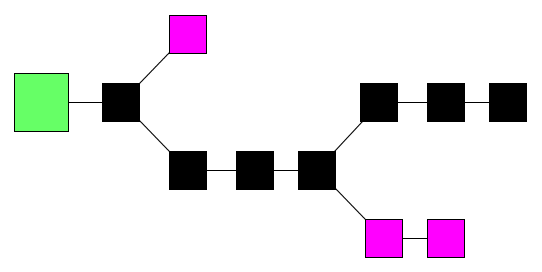
\includegraphics[width=9cm]{blockchain.png}
        \caption[Rappresentazione grafica di una Blockchain]{Rappresentazione grafica di una Blockchain. In verde il nodo iniziale, in nero la catena principale e in viola le diramazioni orfane.}
    \end{figure}

    Le blockchain sono condivise all'interno di reti \textit{peer-to-peer} in cui i vari nodi della rete possiedono una copia integrale o parziale della catena ed utilizzano dei protocolli comuni per la comunicazione con altri nodi e per la validazione e inserimento di nuovi blocchi.
    \\\\
    Una blockchain non è necessariamente immutabile in quanto l'inserimento concorrente di blocchi diversi da parte di nodi diversi della rete sulla stessa catena può creare spesso \textit{fork} ovvero diramazioni ugualmente valide.\\
    Per rendere la blockchain immutabile, man mano che la catena si propaga nella rete e i vari nodi prendono coscienza dell'avvenuto \textit{fork}, un algoritmo condiviso assegna un punteggio ad ogni diramazione in base alle caratteristiche dei blocchi pubblicati e tutti i nodi saranno costretti ad inserire nuovi blocchi sul ramo con punteggio più alto. Nel corso del tempo, il punteggio di una delle diramazioni diventerà molto più alto rispetto a quello delle avversarie e si distingueranno così una diramazione principale e delle diramazioni \textit{orfane} che non verranno più utilizzate in futuro.

    \subsection{Bitcoin}

    \begin{figure}[h!]
        \centering
        
\includegraphics[width=4cm]{bitcoin-logo.png}
        \caption{Logo di \textbf{Bitcoin}}
    \end{figure}

    La blockchain descritta nella sezione precedente [\autoref{contesto:blockchain:struttura}] è stata presentata da Satoshi Nakamoto nel 2008 \cite{nakamoto2008bitcoin} il quale ne ha proposto l'uso al fine di registrare le transazioni della crypto-valuta \textbf{Bitcoin} da un portafoglio virtuale ad un altro.
    \\\\
    Il protocollo di validazione e inserimento di un blocco nella catena è chiamato \textbf{Hashcash} e si basa sul concetto di \textbf{Proof-of-Work}: un \textit{nonce} (che sta per \textit{number used once}) viene aggiunto ad una \textit{base string} al fine di trovare un hash esadecimale che sia minore di un valore \textit{target} (si veda l'esempio in \autoref{img:hashcash}). Vista la bassa probabilità di generare velocemente un hash soddisfacente, non è predicibile quale nodo della rete sarà il prossimo a validare ed inserire per primo il blocco nella catena.

    \begin{figure}[h!]
        \centering
%        \hspace*{-3cm}
        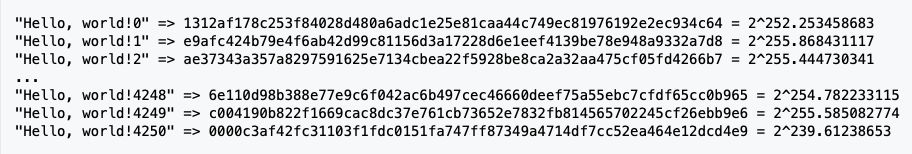
\includegraphics[width=13.5cm]{hashcash.png}
        \caption[Esempio di algoritmo Hashcash]{Esempio di algoritmo \textbf{Hashcash}. Dopo 4251 iterazioni viene trovato il \textit{nonce} che vari la \textit{base string} in modo da ottenere un hash minore del \textit{target} di 2\textsuperscript{240}.}
        \label{img:hashcash}
    \end{figure}

\newpage

%**************************************************************
\section{Ethereum}

\begin{figure}[h!]
    \centering
    
\includegraphics[width=10cm]{ethereum-logo.png}
    \caption{Logo di \textbf{Ethereum}}
\end{figure}

    \subsection{Scopo}
    \textbf{Ethereum} offre tutto ciò che viene offerto da Bitcoin grazie ad una blockchain che sta alla base della crypto-valuta \textbf{ether} ma con un obiettivo molto diverso.
    \\\\
    Bitcoin è stata creata con lo specifico intento di mettere a disposizione una valuta la cui stabilità e legalità non venissero controllate dalle banche centrali e rispettive nazioni ma fossero garantite da un sistema informatico distribuito totalmente indipendente da istituzioni centralizzate. Per fare ciò, Bitcoin si basa sulla blockchain precedentemente descritta [\autoref{contesto:blockchain}] e su un linguaggio di scripting molto limitato, \textit{stack-based}, intenzionalmente \textit{\textbf{non}-Turing-completo} (senza loop) chiamato \textbf{Script}, necessario solo per registrare le transazioni decidendo, quindi, come gli utenti possono accedere alla rete Bitcoin ed utilizzarne la valuta.
    \\\\
    Ethereum, invece, permette di salvare dati arbitrari, rappresentati da una \textit{tupla chiave-valore}, nei propri blocchi e mette a disposizione un linguaggio di programmazione \textit{general-purpose}, \textit{Turing-completo} chiamato \textbf{Solidity} che consente di programmare la blockchain ed utilizzarla come un unico grande computer distribuito. Come Bitcoin, Ethereum è una macchina a stati ma, a differenza di Bitcoin, invece di tener solamente traccia di chi possiede la crypto-valuta, ad ogni transizione viene tracciato il cambio di stato delle tuple chiave-valore. Sulla base del codice caricato, il cambio di stato viene effettuato dalla \textbf{EVM} (Ethereum Virtual Machine) data dalla potenza di calcolo dei nodi sulla rete. Ethereum, dunque, tiene in memoria codice e dati di un software \textit{general-purpose}, esegue il codice e usa la blockchain per tener traccia dei cambiamenti sui dati. Si differenzia da un normale computer (oltre che per la condivisione e immutabilità del registro delle transizioni dato dalla blockchain) in quanto il passaggio di stato deve essere approvato da tutti i nodi presenti sulla rete.\\
    A questo punto, è chiaro che la valuta ether non sia il focus principale di questa tecnologia ma venga principalmente utilizzata come pagamento per i nodi che eseguono il codice e mantengono la blockchain.

    \subsection{Struttura di uno smart contract}
    Uno \textbf{smart contract} è un programma realizzato per essere eseguito dalla blockchain. In termini di programmazione ad oggetti, lo smart contract può essere pensato come una classe contenente dei campi dati privati (stato del contratto), dei metodi pubblici getter/setter per poter accedere/modificare questi dati e altri metodi pubblici per altro genere di computazione.

    \begin{lstlisting}[language=Solidity]
pragma solidity 0.6.11;

contract VendingMachine {

    // Declare state variables of the contract
    address public owner;
    mapping (address => uint) public cupcakeBalances;

    // When 'VendingMachine' contract is deployed:
    // 1. set the deploying address as the owner of the contract
    // 2. set the deployed smart contract's cupcake balance to 100
    constructor() public {
        owner = msg.sender;
        cupcakeBalances[address(this)] = 100;
    }

    // Allow the owner to increase the smart contract's cupcake balance
    function refill(uint amount) public {
        require(msg.sender == owner, "Only the owner can refill.");
        cupcakeBalances[address(this)] += amount;
    }

    // Allow anyone to purchase cupcakes
    function purchase(uint amount) public payable {
        require(msg.value >= amount * 1 ether, "You must pay at least 1 ETH per cupcake");
        require(cupcakeBalances[address(this)] >= amount, "Not enough cupcakes in stock to complete this purchase");
        cupcakeBalances[address(this)] -= amount;
        cupcakeBalances[msg.sender] += amount;
    }
}
    \end{lstlisting}

    Il valore contenuto nei campi dati verrà salvato ad ogni esecuzione mediante l'aggiunta di un blocco sulla catena.

    \subsection{Turing-completness e terminazione}
    \label{contesto:ethereum:terminazione}
    Gli \textbf{smart contract} sono programmati in un linguaggio \textit{Turing-completo} e non si è, quindi, in grado di dimostrare formalmente se giungeranno a terminazione. In un sistema hardware locale, come un PC o una stampante, la cosa genera problemi relativamente limitati in quanto potrebbe essere sufficiente resettare i dispositivi a livello hardware qualora il loro software fosse entrato in un loop infinito. La questione della terminazione non è, invece, così banale nella blockchain Ethereum a cui non può essere semplicemente "staccata la spina".
    \\\\
    Al fine, dunque, di garantire la terminazione dello smart contract viene introdotto un meccanismo di esecuzione "a consumo" basato su una metrica chiamata \textbf{gas}.

    \begin{figure}[h!]
        \centering
        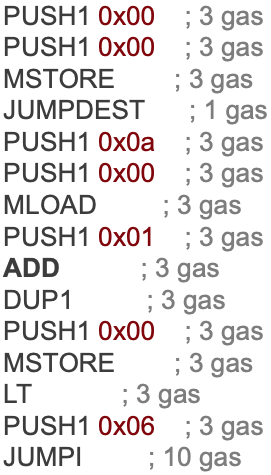
\includegraphics[width=4cm]{gas-eval.png}
        \caption{Ad ogni \textit{OPCODE} viene associato un costo in gas}
    \end{figure}

    Ad ogni istruzione viene assegnato un costo in gas in base al suo costo computazionale. Ad ogni richiesta di esecuzione di una funzione su smart contract che ne modifichi lo stato, il richiedente dichiara quante unità di gas sia disposto a consumare e quanti ether sia disposto a pagare per ogni unità. Un nodo della rete accetta la transazione ed esegue la funzione richiesta. Qualora la funzione termini la quantità di gas messa a disposizione dal richiedente (perché il valore scelto è troppo basso o si è entrati in un loop infinito) l'esecuzione viene conclusa forzatamente garantendo così in ogni caso la terminazione.

%**************************************************************
\section{Token ERC-20}
    \subsection{Scopo}
    Nel corso del tempo si sono sviluppati degli standard per smart contract al fine di semplificare la realizzazione di applicativi decentralizzati. In termini pratici e più vicini alla programmazione ad oggetti, gli standard vanno a definire un interfaccia che verrà poi implementata da uno smart contract "concreto".
    \\\\
    Uno di questi standard è \textbf{ERC-20} che permette la creazione di un \textbf{Fungible Token}. Un token è un "gettone" virtuale che può rappresentare un qualsiasi bene virtuale o materiale come ad esempio: un biglietto della lotteria, un asset finanziario, un punto reputazione in un videogioco online, un kg di oro, ecc.
    Il token ERC-20 è \textit{fungibile} ovvero privo di una individualità specifica e pertanto passibile di sostituzione e scambio. Ogni token, ricavato da uno smart contract conforme a questo standard, ha, dunque, la proprietà di essere uguale per tipologia e valore ad ogni altro token dello stesso smart contract.

    \subsection{Uniswap}
    \label{context:ethereum:uniswap}
    Nel mercato tradizionale, lo scambio di beni avviene tramite gli \textit{order book} che contengono le offerte di scambio aperte divise per chi compra e chi vende un determinato bene. Una transazione viene eseguita quando venditore e acquirente riescono ad accordarsi sul suo prezzo.\\
    Per esempio: supponiamo che Luca voglia vendere il bene X a un prezzo di \euro{2,30} mentre Anna voglia comprare il bene X al prezzo di \euro{2,20}. Luca e Anna a questo punto hanno due possibilità: aspettare che altri trader si accordino al loro prezzo oppure "venirsi incontro" decidendo rispettivamente di vendere a prezzo più vantaggioso e comprare a prezzo più alto delle stime iniziali (accordandosi ad esempio su \euro{2,25}).
    Se volessimo applicare questa procedura allo scambio di token fungibili, mediante appositi smart contract che fungano da order book, il sistema scalerebbe molto faticosamente: gli algoritmi preposti ad elaborare grandi moli di dati richiedono, infatti, molto gas per il solo scorrimento delle strutture dati alla ricerca di un match, con il rischio tangibile che l'algoritmo si interrompa prima della sua conclusione, come precedentemente discusso [\autoref{contesto:ethereum:terminazione}].

    \begin{figure}[h!]
        \centering
        
\includegraphics[width=4cm]{uniswap-logo.png}
        \caption{Logo di \textbf{Uniswap}}
    \end{figure}

    \textbf{Uniswap} è un applicativo decentralizzato, rilasciato su Ethereum, che permette lo scambio di token fungibili senza utilizzare il modello degli order book. Per farlo mette a disposizione delle \textbf{liquidity pool} ovvero dei contenitori virtuali per i due token di cui si vuole permettere lo scambio. Quest'ultimo, quindi, non avverrà più fra due trader ma fra il trader e la liquidity pool (ovvero con uno smart contract).
    \\\\
    L'exchange rate (a meno della fee in ether per coprire i costi di gas) viene stabilito automaticamente sulla base della relazione:
    \[
    nTokenA \times nTokenB = k
    \]
    dove \textit{nTokenA} e \textit{nTokenB} sono le quantità dei due token presenti nella liquidity pool e \textit{k} è una costante che viene decisa al momento del deposito della liquidità iniziale di token A e B.

    \subsection{wETH}
    La crypto-valuta \textbf{ether} (rappresentata anche come \textbf{ETH}), al pari di tutte le valute, si comporta esattamente come un token fungibile con la differenza che essendo alla base della blockchain Ethereum non è conforme allo standard ERC-20 che è stato definito dopo di essa. Per ovviare al problema è stato successivamente creato \textbf{wETH} (sta per Wrapped ETH) con lo scopo di permettere lo scambio (con sistemi come Uniswap [\autoref{context:ethereum:uniswap}]) fra crypto-valuta ETH e un qualsiasi altro fungible token.\\
    Si noti come, così come wETH, esistono altri token \textit{wrapper} riferiti a valute legali o altre crypto-valute come \textbf{WBTC} per Bitcoin.

    \subsection{Il token Sync Lab}
    L'azienda Sync Lab sta portando avanti un progetto di ricerca interno sullo studio di token fungibili mantenuti da un infrastruttura decentralizzata. Come risultato di questa ricerca sta prendendo forma un token basato su ERC-20 che rappresenta il valore di oggetti disponibili all'acquisto in una vetrina di un portale di e-commerce.

\newpage

\section{Node.js}
Vincolo di progetto è quello di utilizzare \textbf{Node.js} come piattaforma per l'esecuzione del back-end. Node.js è un interprete per linguaggio \textbf{JavaScript} che ha acquisito fama al pari di \textbf{Java} come tecnologia per la creazione di applicazioni web. Una breve ricerca sulla rete ricondurrà questo successo ad alcune caratteristiche fondamentali:
\begin{itemize}
    \item JavaScript nasce per essere un linguaggio semplice per la creazione di pagine web dinamiche anche da parte dei non esperti il che lo rende generalmente meno verboso di Java;
    \item gli artefatti Node.js sono tendenzialmente più piccoli di quelli Java il che non aumenta esponenzialmente la crescita dovuta alle dipendenze;
    \item il sofware Node è decisamente più snello della JVM inclusa con il JDK:\\
    Node $\approx$ 30MB vs.\ JDK $\approx$ 110MB; ciò rende la containerizzazione più agevole e il software più scalabile in caso di architettura a microservizi;
    \item arriva out-of-the-box con il sistema di gestione delle dipendenze \textbf{npm}.
\end{itemize}
È risultato, dunque, d'interesse per Sync Lab capire se vi fossero peculiarità legate all'applicazione di questa tecnologia in questo contesto. Essendo il caso d'uso dell'e-commerce abbastanza comune, è opportuno scegliere un framework per Node.js che permetta di non "reinventare la ruota" e programmare efficientemente [\autoref{tech:adonis}].

\section{Un e-commerce basato su token fungibili}
Bitcoin mette a disposizione una moneta che non obblighi il proprio utilizzatore a dare fiducia alle istituzioni (inter)nazionali per garantirne legalità e stabilità. È ragionevole pensare che crypto-valute e relative blockchain siano qui per restare e in tale contesto è utile studiare soluzioni che siano in grado di farne buon uso. Da qui nasce l'idea di un e-commerce basato su token fungibili che abbia le seguenti caratteristiche:
\begin{itemize}
    \item utilizzo semplice per chi già possiede crypto-valuta grazie alla facilità di scambio fra essa e token mediante Uniswap;
    \item anonimato garantito (per chi ne volesse fruire) dato dalla mancata associazione fra un wallet e una persona fisica (il wallet può essere usato da chiunque ne conosca la chiave privata);
    \item avere a disposizione un registro condiviso ed immutabile in cui siano verificabili le transazioni effettuate con il negozio virtuale.
\end{itemize}

\newpage

\section{Struttura dell'e-commerce}
    \subsection{Struttura Dapp tipica}
    La struttura tipica di una \textbf{Dapp} (applicazione decentralizzata) basata su blockchain Ethereum prevede che il back-end sia totalmente realizzato mediante smart contract mentre il front-end sia un applicazione grafica in JavaScript (o TypeScript) eseguibile da browser web che comunichi con un nodo della rete Ethereum tramite un'apposita libreria come \textbf{web3.js}.

    \begin{figure}[h!]
        \centering
%        \hspace*{-2cm}
        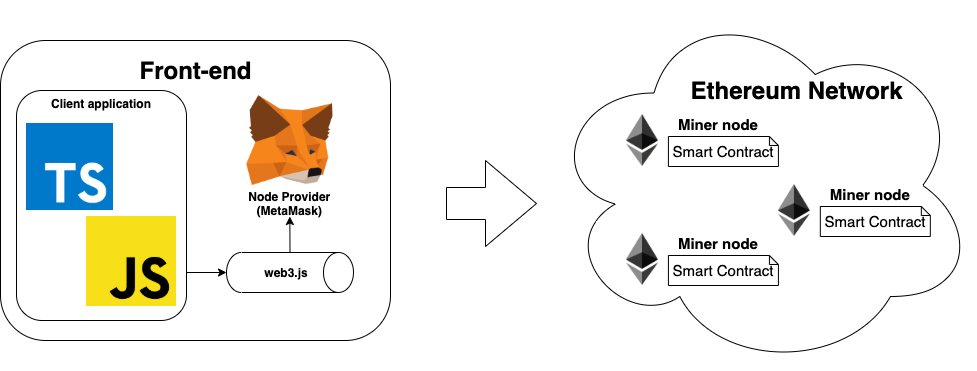
\includegraphics[width=13.5cm]{dapp-diagram.png}
        \caption{Struttura tipica di un'applicazione decentralizzata}
    \end{figure}

    Mettere in piedi un nodo della rete Ethereum risulta poco pratico in termini di risorse e potenza computazionale (ogni nodo contiene al suo interno tutta la blockchain) dunque web3.js comunica con la rete Ethereum tramite \textbf{MetaMask} che funge da \textit{node provider} oltre a mettere a disposizione la gestione grafica dei propri \textit{wallet} Ethereum [\autoref{img:wallet}] e delle transazioni verso altri wallet o verso funzioni degli smart contract che implichino un loro cambio di stato [\autoref{img:transaction}].

    \begin{figure}[p]
        \centering
        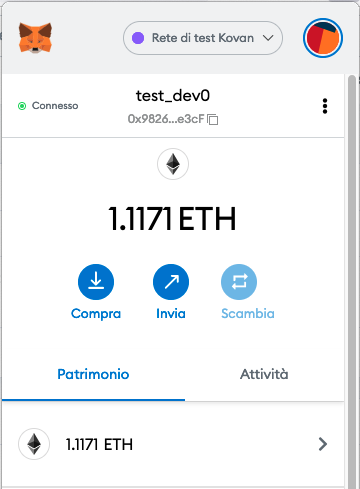
\includegraphics[width=5cm]{metamask-wallet.png}
        \caption{\textbf{MetaMask} per la gestione di un wallet Ethereum da browser web}
        \label{img:wallet}

        \centering
        \hspace*{-1cm}
        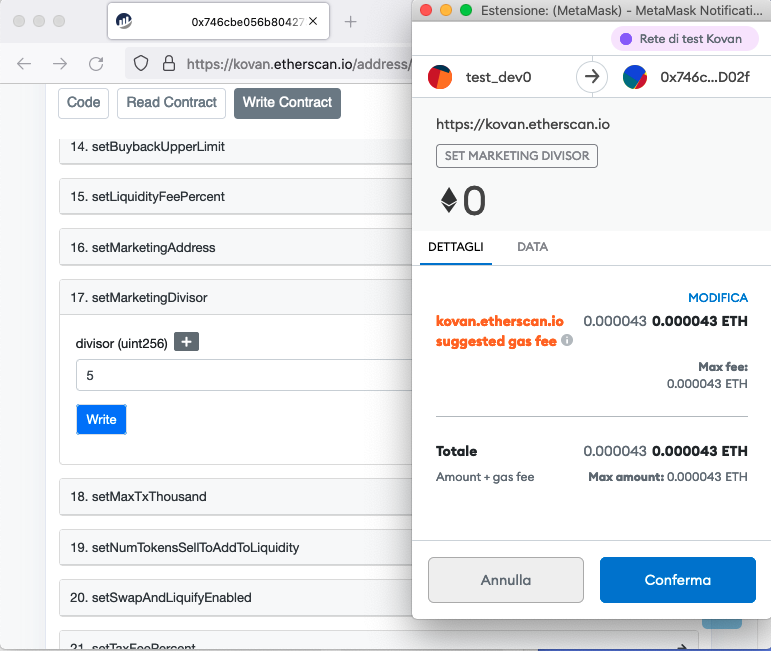
\includegraphics[width=14.5cm]{metamask-transaction.png}
        \caption{\textbf{MetaMask} per la gestione di una transazione verso un smart contract}
        \label{img:transaction}
    \end{figure}

    \subsection{Integrazione Dapp con back-end tradizionale}
    \label{context:structure:dapp-backend}
    Durante la discussione dell'idea di progetto con tutor esterno e project manager, si è concluso che la struttura tipica di una Dapp non fosse adatta al caso d'uso di un e-commerce basato su token. Il motivo principale sta nel fatto che la manipolazione di dati all'interno della blockchain, implicandone un cambiamento di stato, ha un costo in gas. Alcune operazioni basilari all'interno di un e-commerce potrebbero essere: registrazione utente, modifica dati utente, inserimento nuovo prodotto, modifica prezzo prodotto, creazione nuovo ordine, cambio di stato dell'ordine (es. da "spedito" a "consegnato"), ecc. Tutte le operazioni precedentemente descritte hanno un costo che deve essere assorbito dall'e-commerce o addirittura dall'utente! Si ritiene che ciò sia inaccettabile anche considerato che, per esperienza interna a Sync Lab, nell'anno corrente il costo del gas è elevato e la somma dei costi per le operazioni arriverebbe molto probabilmente a superare i prezzi per un hosting su cloud o per mantenimento di un server interno.
    \\\\
    Si è, dunque, deciso di inserire all'interno della struttura un back-end tradizionale con annesso database relazionale [\autoref{img:dapp-backend}] che funga da gestore per utenti, prodotti, ordini e relativi dati oltre ad essere il punto principale di comunicazione con la rete Ethereum per gestione e pagamenti mediante lo smart contract ERC-20 riguardante il token di Sync Lab. Questo documento descrive la realizzazione di tale back-end.
    \\\\
    L'accesso alla Dapp non rimane, però, esclusivo al back-end. Il front-end, infatti, oltre ad interagire con il back-end tramite \textbf{API REST}, comunica (tramite MetaMask) con lo smart contract del token al fine di:
    \begin{itemize}
        \item permettere l'acquisto di token mediante Uniswap;
        \item garantire l'integrazione fra wallet Ethereum e utenza dell'ecommerce;
        \item approvare il prelievo di token dal proprio wallet, pari all'importo dell'ordine,  da parte del back-end mediante la function \textsc{approve} messa a disposizione dall'interfaccia ERC-20.
    \end{itemize}
    \begin{lstlisting}[language=Solidity]
function approve(address _spender, uint256 _value) public returns (bool success)
    \end{lstlisting}

    \begin{figure}[p]
        \centering
        \hspace*{-2cm}
        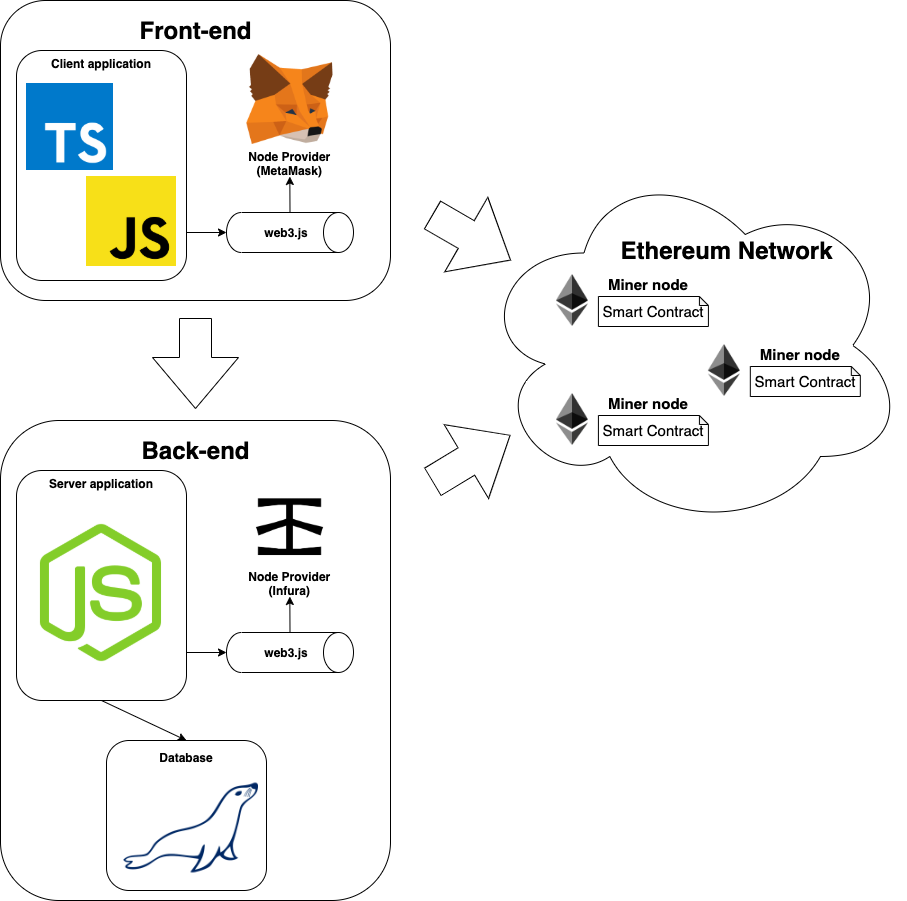
\includegraphics[width=17cm]{dapp-backend-diagram.png}
        \caption{Struttura che integra un applicativo decentralizzato e un app con back-end tradizionale}
        \label{img:dapp-backend}
    \end{figure}